%-- Section : GoT introductory presentation --%
\section{The Games on Track (GoT) System}
One available system for a start is the \emph{Games on Track GT-Position} (see \appref{GoTDescription}) system which is able to determine the lawn mower's position in space.\\
%
It is composed of four different parts both hardware and software \cite{GOTWebsitePos} :
\begin{itemize}
	\item A tracked module, which emits ultra-sound waves. It should be placed on the lawn mower itself while taking care, that the emitting cell is not obstructed by anything.
	\item Beacons or receivers, placed around the area the lawn mower will move in. Depending on the terrain, anywhere from 2 to more than 20 of these can be used: the more is placed, the more accuracy can be obtained to fight against any ambient noise, or the more space can be monitored.
	\item The central system, which calculates the distance of the tracked module to each beacon, and transmits it to the computer via USB in regular intervals.
	\item The GoT software aggregates the received positions throughout time, and can be used to draw a map of the terrain (the lawn), and to determine the absolute position of the tracked module.
\end{itemize}

\begin{figure}[H]
\centering
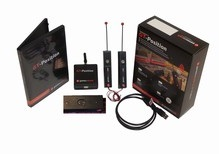
\includegraphics[scale=1.1]{figures/gotSystem.jpg} 
\caption{Games on Track GT-Position package [source:Games\ on\ Track]} 
\label{fig:gotsystem}
\end{figure}
\noindent

GoT was originally designed for train modelling, but it is easily adaptable for any use of position tracking and seems a good choice, at first, for a basic autonomous lawn mower.
But, why not use a satellite based positioning system ?
